\subsection{Плоска област на Скот}

\Stefan{По принцип плоската област на Скот се дефинира върху друга област на Скот}

Да фиксираме едно произволно непразно множество $A$ и един елемент $\bot \not \in A$.
Да означим $A_\bot = A \cup \{\bot\}$ и да разгледаме следната бинарна релация $\sqsubseteq$ върху $A_\bot$:
\[a \sqsubseteq b\ \iff\ a = \bot\ \vee\ a = b.\]
Лесно се съобразява, че $\sqsubseteq$ задава {\em частична наредба} върху $A_\bot$:
\marginpar{От деф. на $\sqsubseteq$ следва, че $\bot$ е най-малкият елемент}
\begin{itemize}
\item 
  {\em рефлексивност}: $a \sqsubseteq a$ за всяка $a \in A_\bot$;
\item
  {\em транзитивност}: $a \sqsubseteq b\ \&\ b \sqsubseteq c \implies a\sqsubseteq c$ за всеки $a,b,c \in A_\bot$;
\item
  {\em антисиметричност}: $a \sqsubseteq b\ \&\ b\sqsubseteq a \implies a = b$ за всеки $a,b \in A_\bot$.
\end{itemize}

Наредбата $(A_\bot, \sqsubseteq)$ ще наричаме {\bf плоска наредба}. Тя ще играе важна роля в нашите разглеждания.
\marginpar{$\bot$ се нарича {\em bottom} елемент}
Например, често ще разглеждаме плоската наредба $(\Nat_\bot, \sqsubseteq)$.

\begin{framed}
  \begin{figure}[H]
    \label{fig:flat-nat-1}
    \centering
    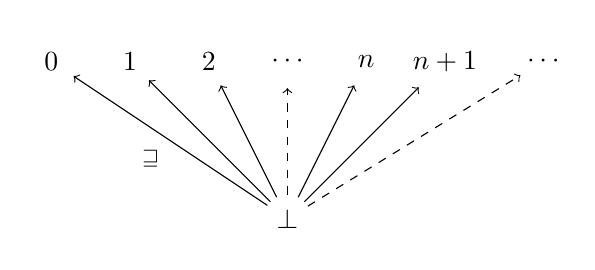
\begin{tikzpicture}[shorten >=1pt,->]
      \tikzstyle{vertex}=[circle,minimum size=17pt,inner sep=0pt]
      
      \node[vertex] (bot) at (3,0) {$\bot$};
      \node[vertex] (0) at (0,2) {$0$};
      \node[vertex] (1) at (1,2) {$1$};
      \node[vertex] (2) at (2,2) {$2$};
      \node[vertex] (dots) at (3,2) {$\cdots$};
      \node[vertex] (n) at (4,2) {$n$};
      \node[vertex] (n1) at (5,2) {$n+1$};
      \node[vertex] (ddots) at (6.25,2) {$\cdots$};
      
      \draw (bot) -- node[below left]{$\scriptstyle{\sqsupseteq}$} (0);
      \draw (bot) -- (1);
      \draw (bot) -- (2);
      \draw[dashed] (bot) -- (dots);
      \draw (bot) -- (n);
      \draw (bot) -- (n1);
      \draw[dashed] (bot) -- (ddots);
    \end{tikzpicture}    
    \caption{Графично представяне на плоската наредба $\sqsubseteq$ върху $\Nat_\bot$}
  \end{figure}
  \end{framed}

\begin{proposition}
  \index{област на Скот!плоска}
  Нека $A$ е произволно множество и нека елементът $\bot \not \in A$.
  \marginpar{На англ. {\em flat domain}}
  Определяме наредената тройка $\A_\bot = (A_\bot, \sqsubseteq, \bot)$ като:
  \begin{itemize}
  \item 
    $A_\bot = A\cup\{\bot\}$;
  \item
    $\sqsubseteq$ задава {\em плоската наредба} върху $A_\bot$.
  \end{itemize}
  Тогава $\A_\bot$ е област на Скот, която ще наричаме {\bf плоска област на Скот} за множеството $A$.
\end{proposition}

%%% Local Variables:
%%% mode: latex
%%% TeX-master: "../sep"
%%% End:
